\section{Case Study: Shopping Carts}
\label{sec:carts}

\jmh{All the above is only interesting if it helps programmers write intuitive code with a minimum of coordination.  Say something to motivate the case studies as a critical part of the paper.  Two plausible goals: (1) show that the use of lattices lets us remove apparent points of order from previous Bloom programs.  (2) show that the use of \lang and its lattices is a good match to distributed systems programming.}

\begin{figure}[t]
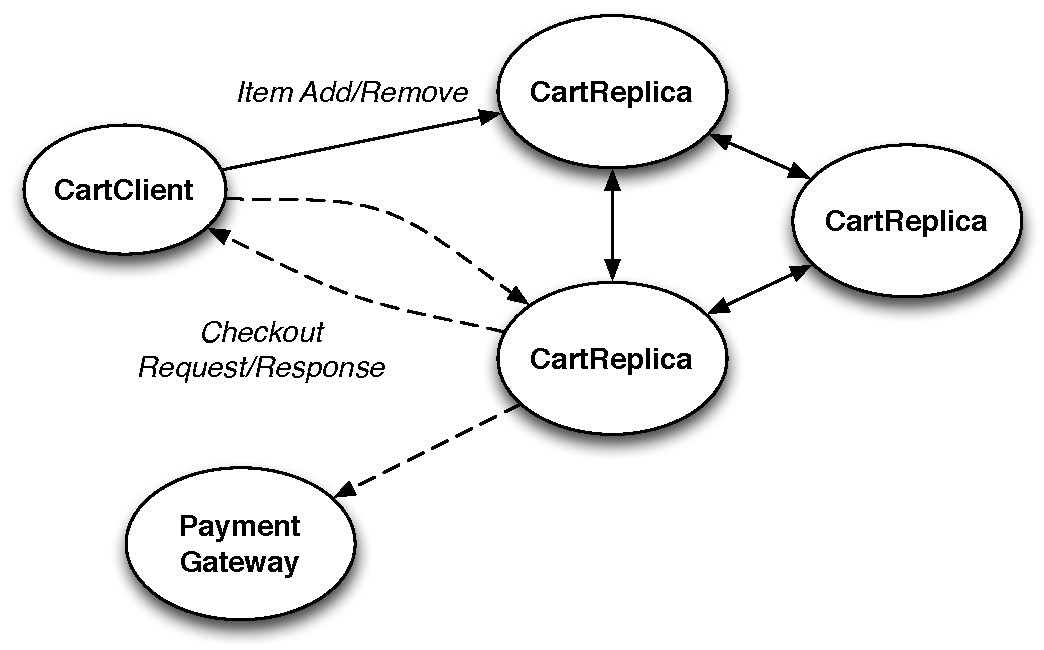
\includegraphics[width=\linewidth]{fig/cart_arch.pdf}
\label{fig:cart-system}
\caption{Architecture of a simple shopping cart system.}
\end{figure}

In this section, we consider a simple e-commerce system in which clients
interact with a shopping cart service, adding and removing items over the course
of a browsing session (Figure~\ref{fig:cart-system}). The shopping cart service
is replicated to improve fault tolerance; client requests can be routed to any
of the cart replicas. Eventually, a client submits a ``checkout'' operation, at
which point the cumulative effect of their shopping session should be summarized
and returned to the client. In a more complete system, the result of the
checkout operation might be presented to the client for confirmation or
submitted to a payment processor to complete the e-commerce transaction. This
case study is based on the cart system from Alvaro et al.~\cite{Alvaro2011},
which was in turn inspired by the discussion of replicated shopping carts in the
Dynamo paper~\cite{DeCandia2007}.

Alvaro et al.\ consider two different cart designs: a ``disorderly'' version in
which the cart state is represented as a set of operations (allowing monotonic
accumulation of adds and removes) and a ``destructive'' version in which the
cart state is managed by a key-value store, which requires a non-monotonic
update on each cart action. In both designs, Alvaro et al.\ argue that the
checkout operation is non-monotonic because it requires aggregating over all
previous operations applied to the cart.

In this section, we use \lang to make two improvements to the cart
service. First, we improve the ``destructive'' design by using lattices to make
updates to the key-value store monotonic. Second, we show that lattices can be
used to make the checkout process monotonic. In both cases, the result is a
reduced need for coordination and more confidence in the eventual
consistency/convergence of the cart system.

\subsection{Monotonic Destructive Cart}
TODO: basic idea is that if we fix the set of replicas, we can do ``early
summaries'' of cart actions---i.e., convert the operation log format into the
format used by the naive destructive cart, once we know that a given operation
has reached all replicas. Is this worth including?

\subsection{Monotonic Checkout}
Alvaro et al.\ argue that processing a checkout request is non-monotonic because
it requires aggregating over an asynchronously computed data set; in general,
coordination might be required to ensure that the complete input has been
received before the checkout request can be processed correctly. However, note
that the client knows exactly which add/remove operations should be reflected in
the result of the checkout; if that information can be propagated to the cart
service, any chosen replica can decide if it has enough information to process
the checkout operation without needing to coordinate.

This can be done by assigning IDs to each message sent by the client. Each
client has a session ID; within a session, operation IDs are assigned in
increasing numeric order without gaps. Hence, if the client sends a ``lower
bound'' operation ID along with the checkout message, any replica of the cart
service can independently ensure that it only produces a response message once
it has received all the operations in the ID range indicated by the client. This
essentially requires a threshold test over the operation IDs received by a given
replica, which can easily be implemented using \lang.

% Note that because each replica determines when the cart is ``complete''
% independently, multiple response messages may be produced. However, they will
% all be consistent, because ...

% \subsection{Performance Study}
% \begin{itemize}
% \item
%   goal: demonstrate that removing coordination from a distributed protocol can
%   significantly reduce its running time
% \item
%   benchmark: destructive cart w/ coordination on each action vs.\ destructive
%   cart in \lang without coordination, disorderly cart with coordination on
%   checkout vs.\ disorderly cart with monotonic checkout
% \end{itemize}
